\documentclass[12pt]{beamer}
\usepackage{../Estilos/BeamerMAF}
\usepackage[absolute, overlay]{textpos}
\usepackage{../Estilos/ColoresLatex}
\usetheme{Copenhagen}
\usecolortheme{wolverine}
%\useoutertheme{default}
\setbeamercovered{invisible}
% or whatever (possibly just delete it)
\setbeamertemplate{section in toc}[sections numbered]
\setbeamertemplate{subsection in toc}[subsections numbered]
\setbeamertemplate{subsection in toc}{\leavevmode\leftskip=3.2em\rlap{\hskip-2em\inserttocsectionnumber.\inserttocsubsectionnumber}\inserttocsubsection\par}
% \setbeamercolor{section in toc}{fg=blue}
% \setbeamercolor{subsection in toc}{fg=blue}
% \setbeamercolor{frametitle}{fg=blue}
\setbeamertemplate{caption}[numbered]

\setbeamertemplate{footline}
\beamertemplatenavigationsymbolsempty
\setbeamertemplate{headline}{}


\makeatletter
% \setbeamercolor{section in foot}{bg=gray!30, fg=black!90!orange}
% \setbeamercolor{subsection in foot}{bg=blue!30}
% \setbeamercolor{date in foot}{bg=black}
\setbeamertemplate{footline}
{
  \leavevmode%
  \hbox{%
  \begin{beamercolorbox}[wd=.333333\paperwidth,ht=2.25ex,dp=1ex,center]{section in foot}%
    \usebeamerfont{section in foot} \insertsection
  \end{beamercolorbox}%
  \begin{beamercolorbox}[wd=.333333\paperwidth,ht=2.25ex,dp=1ex,center]{subsection in foot}%
    \usebeamerfont{subsection in foot}  \insertsubsection
  \end{beamercolorbox}%
  \begin{beamercolorbox}[wd=.333333\paperwidth,ht=2.25ex,dp=1ex,right]{date in head/foot}%
    \usebeamerfont{date in head/foot} \insertshortdate{} \hspace*{2em}
    \insertframenumber{} / \inserttotalframenumber \hspace*{2ex} 
  \end{beamercolorbox}}%
  \vskip0pt%
}
\makeatother

\makeatletter
\patchcmd{\beamer@sectionintoc}{\vskip1.5em}{\vskip0.8em}{}{}
\makeatother

% %\newlength{\depthofsumsign}
% \setlength{\depthofsumsign}{\depthof{$\sum$}}
% \newcommand{\nsum}[1][1.4]{% only for \displaystyle
%     \mathop{%
%         \raisebox
%             {-#1\depthofsumsign+1\depthofsumsign}
%             {\scalebox
%                 {#1}
%                 {$\displaystyle\sum$}%
%             }
%     }
% }
% \def\scaleint#1{\vcenter{\hbox{\scaleto[3ex]{\displaystyle\int}{#1}}}}
% \def\scaleoint#1{\vcenter{\hbox{\scaleto[3ex]{\displaystyle\oint}{#1}}}}
% \def\bs{\mkern-12mu}


\setbeamercolor{section in foot}{bg=peridot, fg=black}
\setbeamercolor{subsection in foot}{bg=powderblue(web), fg=black}


\makeatletter
\setbeamertemplate{footline}
{
\leavevmode%
\hbox{%
\begin{beamercolorbox}[wd=.333333\paperwidth,ht=2.25ex,dp=1ex,center]{section in foot}%
  \usebeamerfont{section in foot} \insertsection
\end{beamercolorbox}%
\begin{beamercolorbox}[wd=.333333\paperwidth,ht=2.25ex,dp=1ex,center]{subsection in foot}%
  \usebeamerfont{subsection in foot}  \insertsubsection
\end{beamercolorbox}%
\begin{beamercolorbox}[wd=.333333\paperwidth,ht=2.25ex,dp=1ex,right]{date in head/foot}%
  \usebeamerfont{date in head/foot} \insertshortdate{} \hspace*{1.5em}
  \insertframenumber{} / \inserttotalframenumber \hspace*{2ex} 
\end{beamercolorbox}}%
\vskip0pt%
}
\makeatother
\usefonttheme{serif}
\setbeamercolor{frametitle}{bg=palecerulean}
\resetcounteronoverlays{saveenumi}

\date{19 de mayo de 2022}

\title{\large{El oscilador armónico cuántico}}
\subtitle{Funciones de Hermite}
\author{M. en C. Gustavo Contreras Mayén}

\begin{document}
\maketitle
\fontsize{14}{14}\selectfont
\spanishdecimal{.}

\section*{Contenido}
\frame{\frametitle{Temas a revisar} \tableofcontents[currentsection, hideallsubsections]}

\section{El oscilador cuántico}
\frame{\tableofcontents[currentsection, hideothersubsections]}
\subsection{Enunciado del problema}

\begin{frame}
\frametitle{Por resolver}
\setbeamercolor{item projected}{bg=black,fg=white}
\setbeamertemplate{enumerate items}{%
\usebeamercolor[bg]{item projected}%
\raisebox{1.5pt}{\colorbox{bg}{\color{fg}\footnotesize\insertenumlabel}}%
}
\begin{enumerate}[<+->]
\item Construye la función $\psi_{2} (x)$.
\item De manera directa revisa la ortogonalidad de $\psi_{0}$, $\psi_{1}$ y $\psi_{2}$ mediante la integración explícita.
\end{enumerate}
\end{frame}

\subsection{Herramienta de solución}

\begin{frame}
\frametitle{De las notas de trabajo}
En el material de revisión, se plantea el problema del oscilador armónico cuántico, llegando a la expresión que determina el estado base:
\begin{align*}
\psi_{0} (x) = \bigg( \dfrac{m \omega}{\pi \hbar} \bigg)^{\frac{1}{4}} \, \exp\bigg(- \dfrac{m \omega}{2 \hbar} x^{2} \bigg)
\end{align*}
\end{frame}
\begin{frame}
\frametitle{Operador de ascenso}
Para obtener un estado de orden mayor, ocupamos el operador de ascenso:
\pause
\begin{align*}
\psi_{n} (x) = A_{n} \, (a_{+})^{n} \, \phi_{0} (x)
\end{align*}
donde $A_{n}$ es una constante de normalización.
\end{frame}
\begin{frame}
\frametitle{La constante de normalización}
Al resolver la constante de normalización, tenemos que con el operador de ascenso, el estado del oscilador armónico cuántico es:
\pause
\begin{align*}
\psi_{n} = \dfrac{1}{\sqrt{n!}} \, (a_{+})^{n} \, \psi_{0}
\end{align*}
\end{frame}
\begin{frame}
\frametitle{El operador de ascenso}
El operador de ascenso está dado por:
\pause
\begin{align*}
a_{\pm} = \dfrac{1}{\sqrt{2 \hbar m \omega}} \, \bigg( \hbar \, \dv{x} + m \, \omega \, x \bigg)
\end{align*}
\pause
De tal manera que contamos con los elementos para resolver el inciso que se nos pide.
\end{frame}

\subsection{Solución Inciso 1}

\begin{frame}
\frametitle{Aplicando el operador de ascenso}
Tendremos entonces que:
\pause
\begin{eqnarray*}
\begin{aligned}
&a_{+} \psi_{0} = \dfrac{1}{\sqrt{2 \hbar m \omega}} \bigg( - \hbar \dv{x} + m \omega x \bigg) \bigg( \! \dfrac{m \omega}{\pi \hbar} \bigg)^{\frac{1}{4}} \times \\[0.5em]
&\times \exp\bigg(- \dfrac{m \omega}{2 \hbar} x^{2} \bigg) = \\[0.5em] \pause
\end{aligned}
\end{eqnarray*}
\end{frame}
\begin{frame}
\frametitle{Aplicando el operador de ascenso}
Haciendo la diferenciación y el producto:
\pause
\begin{eqnarray*}
\begin{aligned}
&a_{+} \psi_{0} = \dfrac{1}{\sqrt{2 \hbar m \omega}} \bigg( \dfrac{m \omega}{\pi \hbar} \bigg)^{\frac{1}{4}} \bigg[ - \hbar \bigg( - \dfrac{m \omega}{2 \hbar} \bigg) {+} m \omega x \bigg] \times \\[0.5em]
&\times \exp\bigg(- \dfrac{m \omega}{2 \hbar} x^{2} \bigg) = 
\end{aligned}
\end{eqnarray*}
\end{frame}
\begin{frame}
\frametitle{Aplicando el operador de ascenso}
Obteniendo entonces:
\pause
\begin{align*}
a_{+} \psi_{0} = \dfrac{1}{\sqrt{2 \hbar m \omega}} \bigg( \dfrac{m \omega}{\pi \hbar} \bigg)^{\frac{1}{4}} \, 2 m \omega x \exp\bigg(- \dfrac{m \omega}{2 \hbar} x^{2} \bigg)
\end{align*}
\end{frame}
\begin{frame}
\frametitle{Elevando al cuadrado el operador de ascenso}
Tenemos que tomar el cuadrado del operador de ascenso, así que:
\pause
\begin{align*}
&(a_{+})^{2} \psi_{0} = \dfrac{1}{2 \hbar m \omega} \bigg( \dfrac{m \omega}{\pi \hbar} \bigg)^{\frac{1}{4}} \, 2 m \omega x \bigg( \hbar \, \dv{x} + m \, \omega \, x \bigg) \times \\[0.5em]
&\times \exp\bigg(- \dfrac{m \omega}{2 \hbar} x^{2} \bigg)
\end{align*}
\end{frame}
\begin{frame}
\frametitle{Haciendo las cuentas}
Al resolver la parte de diferenciación y producto, tendremos:
\pause
\begin{align*}
&(a_{+})^{2} \psi_{0} = \dfrac{1}{\hbar} \bigg( \dfrac{m \omega}{\pi \hbar} \bigg)^{\frac{1}{4}} \bigg[ - \hbar \bigg( 1 - x \dfrac{m \omega}{2 \hbar} \bigg) + m \omega x^{2} \bigg] \times \\[0.5em]
&\times \exp\bigg(- \dfrac{m \omega}{2 \hbar} x^{2} \bigg)
\end{align*}
\end{frame}
\begin{frame}
\frametitle{Resultado}
Al simplificar la expresión anterior, llegamos al resultado:
\pause
\begin{align*}
(a_{+})^{2} \psi_{0} = \bigg( \dfrac{m \omega}{\pi \hbar} \bigg)^{\frac{1}{4}} \bigg( \dfrac{2 m \omega}{\hbar} x^{2} - 1 \bigg) \exp\bigg(- \dfrac{m \omega}{2 \hbar} x^{2} \bigg)
\end{align*}
\end{frame}
\begin{frame}
\frametitle{Estado del oscilador armónico}
Ocupando la expresión con la constante de normalización, llegamos al resultado:
\pause
\begin{eqnarray*}
\begin{aligned}
\psi_{2} (x) &= \dfrac{1}{\sqrt{2}} (a_{+})^{2} \, \psi_{0} = \\[0.5em] \pause
&= \dfrac{1}{\sqrt{2}} \, \bigg( \dfrac{m \omega}{\pi \hbar} \bigg)^{\frac{1}{4}} \bigg( \dfrac{2 m \omega}{\hbar} x^{2} - 1 \bigg) \exp\bigg(- \dfrac{m \omega}{2 \hbar} x^{2} \bigg)
\end{aligned}
\end{eqnarray*}
\end{frame}

\subsection{Solución Inciso 2}

\begin{frame}
\frametitle{Revisando las funciones}
Como se nos pide revisar la ortogonalidad de las funciones $\psi_{0}$, $\psi_{1}$ y $\psi_{2}$, \pause nos conviene tener una gráfica de esas funciones para identificar algún punto favorable para resolver el enunciado.
\end{frame}
\begin{frame}
\frametitle{Gráfica de $\psi_{0}$}
\begin{figure}
  \centering
  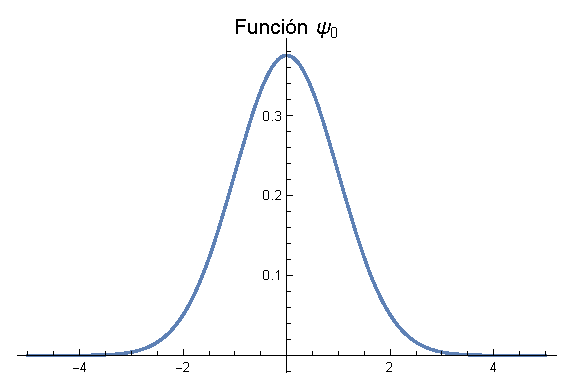
\includegraphics[scale=1]{Imagenes/Plot_Hermite_Psi_0.eps}
\end{figure}
\end{frame}
\begin{frame}
\frametitle{Gráfica de $\psi_{1}$}
\begin{figure}
  \centering
  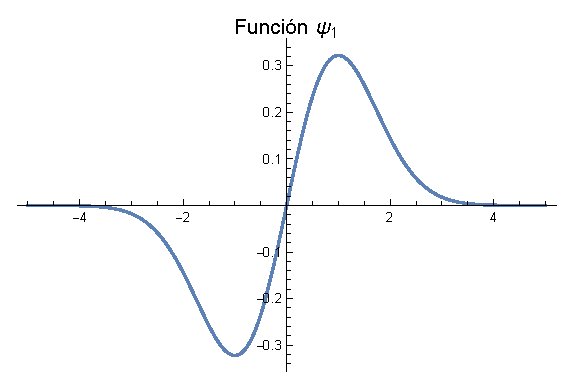
\includegraphics[scale=1]{Imagenes/Plot_Hermite_Psi_1.eps}
\end{figure}
\end{frame}
\begin{frame}
\frametitle{Gráfica de $\psi_{2}$}
\begin{figure}
  \centering
  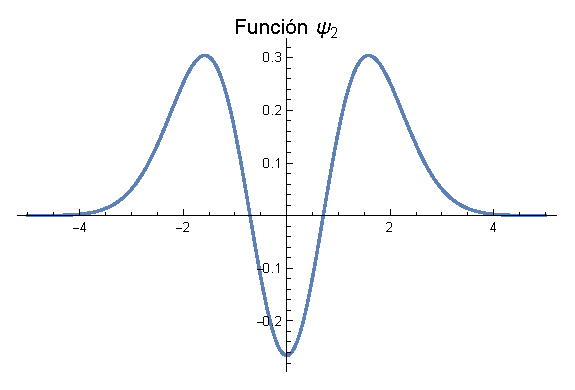
\includegraphics[scale=1]{Imagenes/Plot_Hermite_Psi_2.eps}
\end{figure}
\end{frame}
\begin{frame}
\frametitle{De las gráficas}
Dado que las funciones $\psi_{0}$ y $\psi_{2}$ son \emph{funciones pares}, mientras que $\psi_{1}$ es función impar.
\\
\bigskip
\pause
Las integrales :
\pause
\begin{align*}
\scaleint{6ex} \psi_{0}^{*} \, \psi_{1} \dd{x} \\[0.5em] 
\scaleint{6ex} \psi_{2}^{*} \, \psi_{1} \dd{x} 
\end{align*}
se anulan automáticamente.
\end{frame}
\begin{frame}
\frametitle{La integral a resolver}
Por lo que la única integral que hay que resolver es:
\pause
\begin{eqnarray*}
\begin{aligned}
&\scaleint{6ex} \psi_{2}^{*} \, \psi_{0} \dd{x} = \\[0.5em] \pause
&= \dfrac{1}{\sqrt{2}} \sqrt{\dfrac{m \omega}{\pi \hbar}} \scaleint{6ex}_{\bs -\infty}^{\infty} \bigg( \dfrac{2 m \omega}{\hbar} x^{2} - 1 \bigg) \, \exp\bigg( - \dfrac{m \omega}{\hbar} x^{2} \bigg) =
\end{aligned}
\end{eqnarray*}
\end{frame}
\begin{frame}
\frametitle{Resolviendo la integral}
\begin{align*}
&\scaleint{6ex} \psi_{2}^{*} \, \psi_{0} \dd{x}  = - \sqrt{\dfrac{m \omega}{2 \pi \hbar}} \bigg[ \scaleint{6ex}_{\bs -\infty}^{\infty} \exp\bigg( - \dfrac{m \omega}{\hbar} x^{2} \bigg) \dd{x} + \\[0.5em] 
&- \dfrac{2 m \omega}{\hbar} \scaleint{6ex}_{\bs -\infty}^{\infty} x^{2} \exp\bigg( - \dfrac{m \omega}{\hbar} x^{2} \bigg) \dd{x}  \bigg] =
\end{align*}
\end{frame}
\begin{frame}
\frametitle{Resolviendo la integral}
\begin{eqnarray*}
\begin{aligned}
\scaleint{6ex} \psi_{2}^{*} \, \psi_{0} \dd{x} &= - \sqrt{\dfrac{m \omega}{2 \pi \hbar}} \bigg[ \sqrt{\dfrac{\pi \hbar}{m \omega}} - \dfrac{2 m \omega}{\hbar} \dfrac{\hbar}{2 m \omega} \sqrt{\dfrac{\pi \hbar}{m \omega}} \bigg] = \\[0.5em] \pause
&= 0
\end{aligned}
\end{eqnarray*}
\pause
Se cumple al condición de ortogonalidad entre las funciones del oscilador armónico cuántico.
\end{frame}

\subsection{Ejercicio 2}

\begin{frame}
\frametitle{Enunciado del ejercicio}
Para los estados $\psi_{0}$ y $\psi_{1}$, calcula mediante la integración explícita, los valores esperados:
\pause
\setbeamercolor{item projected}{bg=yellow,fg=black}
\setbeamertemplate{enumerate items}{%
\usebeamercolor[bg]{item projected}%
\raisebox{1.5pt}{\colorbox{bg}{\color{fg}\footnotesize\insertenumlabel}}%
}
\begin{enumerate}[<+->]
\item $\expval{x}$
\item $\expval{p}$
\item $\expval{x^{2}}$
\item $\expval{p^{2}}$
\end{enumerate}
\end{frame}
\begin{frame}
\frametitle{Los valores esperados}
Recordemos que los valores esperados para la posición y el momento, se definen por:
\pause
\begin{eqnarray*}
\begin{aligned}
\expval{x} &= \scaleint{6ex} \Psi^{*} \, x \, \Psi \dd{x} \\[0.5em] \pause
\expval{p} &= m \, \dv{\expval{x}}{t} = \pause \scaleint{6ex} \Psi^{*} \, \bigg( \dfrac{\hbar}{i} \, \pdv{x} \bigg) \, \Psi \dd{x}
\end{aligned}
\end{eqnarray*}
\end{frame}
\begin{frame}
\frametitle{De la paridad de las funciones}
Sabemos que $\psi_{0}$ es una función par, \pause mientras que $\psi_{1}$ es una función impar.
\\
\bigskip
\pause
En este caso, \pause $\abs{\psi}^{2}$ es par.
\end{frame}
\begin{frame}
\frametitle{El valor esperado $\expval{x}$}
Por la razón anterior, tenemos que:
\pause
\begin{eqnarray*}
\expval{x} = \pause \scaleint{6ex} x \, \abs{\psi}^{2} \dd{x} = \pause 0
\end{eqnarray*}
\end{frame}
\begin{frame}
\frametitle{El valor esperado $\expval{p}$}
Se tiene entonces que:
\pause
\begin{eqnarray*}
\expval{p} = \pause m \, \dv{\expval{x}}{t} = \pause 0
\end{eqnarray*}
\pause
\textbf{Nota: } \textcolor{cadetblue}{Estos resultados se mantienen para cualquier estado estacionario del oscilador armónico cuántico.}
\end{frame}
\begin{frame}
\frametitle{Simplificando las operaciones}
Con la finalidad de simplificar las operaciones, \pause ocupemos la siguiente variable:
\pause
\begin{align*}
\xi \equiv \sqrt{\dfrac{m \omega}{\hbar}} x
\end{align*}
\pause
y la constante:
\begin{align*}
\alpha \equiv \bigg( \dfrac{m \omega}{\pi \hbar} \bigg)^{\frac{1}{4}}
\end{align*}
\end{frame}
\begin{frame}
\frametitle{Los estados $\psi_{0}$ y $\psi_{1}$}
De tal manera que los estados para el oscilador armónico, que señala el enunciado son:
\pause
\begin{align*}
\psi_{0} &= \alpha \, \exp\bigg( - \dfrac{\xi^{2}}{2} \bigg) \\[0.5em]
\psi_{1} &= \sqrt{2} \, \alpha \, \xi \, \exp\bigg( - \dfrac{\xi^{2}}{2} \bigg) \\[0.5em]
\end{align*}
\end{frame}
\begin{frame}
\frametitle{Con $n = 0$, el valor esperado $\expval{x^{2}}$}
El valor esperado se encuentra al resolver:
\begin{eqnarray*}
\begin{aligned}
\expval{x^{2}} &= \alpha^{2} \scaleint{6ex}_{\bs \-\infty}^{\infty} x^{2} \xi \, \exp\bigg( - \dfrac{\xi^{2}}{2} \bigg) \dd{x} \\[0.5em] \pause
&= \alpha^{2} \bigg( \dfrac{\hbar}{m \omega} \bigg) \scaleint{6ex}_{\bs -\infty}^{\infty} \xi^{2} \, \exp\big( - \xi^{2} \big) \dd{x} \\[0.5em] \pause
&= \dfrac{1}{\sqrt{\pi}} \bigg( \dfrac{\hbar}{m \omega} \bigg) = \pause \dfrac{\hbar}{2 m \omega}
\end{aligned}
\end{eqnarray*}
\end{frame}
\begin{frame}
\frametitle{Con $n = 0$, el valor esperado $\expval{p^{2}}$}
Ahora para el valor esperado $p^{2}$ en el estado $n = 0$:
\pause
\begin{eqnarray*}
\begin{aligned}
\expval{p^{2}} &= \pause \scaleint{6ex} \psi_{0} \bigg( \dfrac{h}{i} \dv{x} \bigg)^{2} \, \psi_{0} \dd{x} = \\[0.5em] \pause
&= - \hbar^{2} \, \alpha^{2} \sqrt{\dfrac{m \omega}{\hbar}} \scaleint{6ex}_{\bs - \infty}^{\infty} \exp \bigg( - \dfrac{\xi^{2}}{2} \bigg) \dd{x} = \\[0.5em] \pause
&= - \dfrac{m \hbar \omega}{\sqrt{\pi}} \bigg( \dfrac{\sqrt{\pi}}{2} - \sqrt{\pi} \bigg) = \pause \dfrac{m \hbar \omega}{2}
\end{aligned}
\end{eqnarray*}
\end{frame}
\begin{frame}
\frametitle{Con $n = 1$, el valor esperado $\expval{x^{2}}$}
El valor esperado se encuentra al resolver:
\begin{eqnarray*}
\begin{aligned}
\expval{x^{2}} &= 2 \alpha^{2} \scaleint{6ex}_{\bs \-\infty}^{\infty} x^{2} \xi^{2} \, \exp\big( - \xi \big) \dd{x} \\[0.5em] \pause
&= 2 \alpha^{2} \bigg( \dfrac{\hbar}{m \omega} \bigg)^{\frac{3}{2}} \scaleint{6ex}_{\bs -\infty}^{\infty} \xi^{4} \, \exp\big( - \xi^{2} \big) \dd{x} \\[0.5em] \pause
&= \dfrac{2 \hbar}{\sqrt{\pi} m \omega} \, \dfrac{3 \sqrt{\pi}}{4} = \pause \dfrac{3 \hbar}{2 m \omega}
\end{aligned}
\end{eqnarray*}
\end{frame}
\begin{frame}
\frametitle{Con $n = 1$, el valor esperado $\expval{p^{2}}$}
Ahora para el valor esperado $p^{2}$ en el estado $n = 1$:
\pause
\begin{eqnarray*}
\begin{aligned}
\expval{p^{2}} &= - \hbar^{2} \, 2 \, \alpha^{2} \sqrt{\dfrac{m \omega}{\hbar}} \scaleint{6ex}_{\bs - \infty}^{\infty} \exp \bigg( - \dfrac{\xi^{2}}{2} \bigg) \times \\[0.5em]
&\times \bigg[ \dv[2]{\xi} (\xi \exp\bigg( - \dfrac{\xi^{2}}{2} \bigg)) \bigg]  \dd{x} =
\end{aligned}
\end{eqnarray*}
\end{frame}
\begin{frame}
\frametitle{Con $n = 1$, el valor esperado $\expval{p^{2}}$}
\begin{eqnarray*}
\begin{aligned}
\expval{p^{2}} &= - \dfrac{2 m \omega \hbar}{\sqrt{\pi}} \scaleint{6ex}_{\bs - \infty}^{\infty} (\xi^{4} - 3 \xi^{2}) \exp (-\xi^{2}) \dd{\xi} = \\[0.5em] \pause
&= - \dfrac{2 m \omega \hbar}{\sqrt{\pi}} \bigg( \dfrac{3}{4} \sqrt{\pi} - 3 \dfrac{\sqrt{\pi}}{2} \bigg) = \\[0.5em] \pause
&= \dfrac{3 m \hbar \omega}{2}
\end{aligned}
\end{eqnarray*}
\end{frame}

\subsection{Ejercicio 3}

\begin{frame}
\frametitle{Enunciado del ejercicio 3}
Para los estados $\psi_{0}$ y $\psi_{1}$ revisa el principio de incertidumbre.
\end{frame}
\begin{frame}
\frametitle{El principio de incertidumbre}
Recordemos que el principio de incertidumbre, se expresa como:
\pause
\begin{align*}
\sigma_{x} \, \sigma_{p} \geq \dfrac{\hbar}{2}
\end{align*}
\pause
donde $\sigma_{x}$ es la desviación estándar de la posición, y $\sigma_{p}$ es la desviación estándar del momento.
\end{frame}
\begin{frame}
\frametitle{Calculando las desviaciones estándar}
Con el caso $n = 0$, calculamos los valores de $\sigma_{x}$ y $\sigma_{p}$, que obtenemos de las expresiones:
\begin{eqnarray*}
\begin{aligned}
\sigma_{x} &= \pause \sqrt{\expval{x^{2}} - \expval{x}^{2}} = \pause \sqrt{\dfrac{\hbar}{2 m \omega}} \\[0.5em] \pause
\sigma_{p} &= \pause \sqrt{\expval{p^{2}} - \expval{p}^{2}} = \pause \sqrt{\dfrac{m \hbar \omega}{2}}
\end{aligned}
\end{eqnarray*}
\end{frame}
\begin{frame}
\frametitle{El valor del producto}
Con $n = 0$, se tiene entonces que:
\pause
\begin{align*}
\sigma_{x} \, \sigma_{p} = \pause \sqrt{\dfrac{\hbar}{2 m \omega}} \, \sqrt{\dfrac{m \hbar \omega}{2}} = \pause \dfrac{\hbar}{2}
\end{align*}
\pause
Que es correcto en el límite del principio de incertidumbre.
\end{frame}
\begin{frame}
\frametitle{Calculando las desviaciones estándar}
Con el caso $n = 1$, calculamos los valores de $\sigma_{x}$ y $\sigma_{p}$:
\begin{eqnarray*}
\begin{aligned}
\sigma_{x} &= \pause \sqrt{\dfrac{3 \hbar}{2 m \omega}} \\[0.5em] \pause
\sigma_{p} &= \pause \sqrt{\dfrac{3 m \hbar \omega}{2}}
\end{aligned}
\end{eqnarray*}
\end{frame}
\begin{frame}
\frametitle{El valor del producto}
Con $n = 1$, se tiene entonces que:
\pause
\begin{align*}
\sigma_{x} \, \sigma_{p} &= \pause \sqrt{\dfrac{3 \hbar}{2 m \omega}} \, \sqrt{\dfrac{3 m \hbar \omega}{2}} = \\[0.5em] \pause
&= \dfrac{3 \hbar}{2} > \dfrac{\hbar}{2}
\end{align*}
\pause
Cumpliéndose el principio de incertidumbre.
\end{frame}

%Ref. Riley (2006) - 18.9.1
\section{Fórmula de Rodrigues}
\frame{\tableofcontents[currentsection, hideothersubsections]}
\subsection{Demostración}

\begin{frame}
\frametitle{La fórmula de Rodrigues}
De las propiedades para los polinomios de Hermite $H_{n} (x)$, la fórmula de Rodrigues establece que:
\pause
\begin{align*}
H_{n} (x) = (-1)^{n} \exp\big( x^{2} \big) \dv[n]{x} \exp\big( x^{2} \big)
\end{align*}
\pause
Demostremos este resultado.
\end{frame}
\begin{frame}
\frametitle{Haciendo un cambio de variable}
De manera conveniente, hagamos el siguiente cambio de variable:
\pause
\begin{align*}
u =  \exp\big( x^{2} \big)
\end{align*}
\pause
para diferenciar con respecto a $x$, de tal modo que:
\pause
\begin{align*}
\pderivada{u} + 2 \, x \, u = 0
\end{align*}
\end{frame}
\begin{frame}
\frametitle{Diferenciando nuevamente la expresión}
Si diferenciamos esta ecuación $n + 1$ veces, tendremos que:
\pause
\begin{align*}
u^{(n+2)} + 2 \, x \, u^{(n+1)} +  2 \, (n + 1) \, u^{n} = 0
\end{align*}
\end{frame}
\begin{frame}
\frametitle{Otro cambio de variable}
Proponemos ahora el cambio de variable:
\pause
\begin{align*}
v = (-1)^{n} \, u^{(n)}
\end{align*}
\pause
con este cambio, la expresión es:
\pause
\begin{align}
\sderivada{v} + 2 \, x \, v + 2 (n + 1) \, v = 0
\label{eq:ecuacion_18_131}
\end{align}
\end{frame}
\begin{frame}
\frametitle{Otro cambio de variable}
Ahora con el siguiente cambio de variable:
\pause
\begin{align*}
y = \exp\big( x^{2} \big) \, v
\end{align*}
\pause
Tomemos la primera y segunda derivada con respecto a $v$:
\begin{eqnarray*}
\begin{aligned}
\pderivada{y} &= \exp\big( - x^{2} \big) ( \pderivada{y} - 2 \, x \, y) \\[0.5em] \pause
\sderivada{y} &= \exp\big( - x^{2} \big) ( \sderivada{y} - 4 \, x \, \pderivada{y} + 4 \, x^{2} \, y - 2 \, y)
\end{aligned}
\end{eqnarray*}
\end{frame}
\begin{frame}
\frametitle{Usando las derivadas}
Sustituimos las derivadas en la ec. (\ref{eq:ecuacion_18_131}), para luego dividir entre $\exp\big( - x^{2} \big)$, lo que nos lleva a:
\pause
\begin{align*}
\sderivada{y} - 2 \, x \, y + 2 \, n \, y = 0
\end{align*}
\pause
que es la ecuación diferencial de Hermite.
\end{frame}
\begin{frame}
\frametitle{Resultado}
Hemos demostrado que:
\pause
\begin{align*}
y = (-1)^{n} \exp\big( x^{2} \big) \dv[n]{x} \exp\big( - x^{2} \big)
\end{align*}
es solución a la ecuación diferencial.
\\
\bigskip
\pause
Además, dado que esta solución es claramente un polinomio de orden $n$, debe ser algún múltiplo de $H_{n} (x)$.
\end{frame}

\subsection{Ejercicio 4}

\begin{frame}
\frametitle{Enunciado del ejercicio 4}
Usando la fórmula de Rodrigues, calcula $H_{3} (x)$ y $H_{4} (x)$
\end{frame}
\begin{frame}
\frametitle{Calculando las derivadas}
De acuerdo a la fórmula de Rodrigues, \pause se requiere calcular hasta la derivada de orden cuarto de $\exp\big( x^{2} \big)$:
\pause
\begin{eqnarray*}
\begin{aligned}
\dv{x} \bigg( \exp\big( - x^{2} \big) \bigg) &= - 2 \, x \, \exp\big( x^{2} \big) \\[0.5em] \pause
\dv[2]{x} \exp\big( - x^{2} \big) &= \dv{x} \bigg[ - 2 \, x \, \exp\big( x^{2} \big) \bigg] \\[0.5em] \pause
&= \big( -2 + 4 \, x^{2} \big) \exp\big( x^{2} \big)
\end{aligned}
\end{eqnarray*}
\end{frame}
\begin{frame}
\frametitle{Calculando las derivadas}
\begin{eqnarray*}
\begin{aligned}
&\dv[3]{x} \exp\big( - x^{2} \big) = \dv{x} \bigg[ \big( -2 + 4 \, x^{2} \big) \exp\big( x^{2} \big) \bigg] = \\[0.5em] \pause
&= \bigg[ 8 \, x + (-2 + 4 \, x^{2})(- 2 \, x) \bigg] \, \exp\big( - x^{2} \big) = \\[0.5em] \pause
&= (12 \, x - 8 \, x^{3}) \, \exp\big( - x^{2} \big)
\end{aligned}
\end{eqnarray*}
\end{frame}
\begin{frame}
\frametitle{Calculando las derivadas}
\begin{eqnarray*}
\begin{aligned}
&\dv[4]{x} \exp\big( - x^{2} \big) = \dv{x} \bigg[ (12 \, x - 8 \, x^{3}) \, \exp\big( - x^{2} \big) \bigg] = \\[0.5em] \pause
&= \bigg[ 12 - 24 \, x^{2} + (12 \, x - 8 \, x^{3}) (-2 \, x) \bigg] \, \exp\big( - x^{2} \big) = \\[0.5em] \pause
&= (12 \, 48 \, x^{2} + 16 \, x^{4}) \, \exp\big( - x^{2} \big)
\end{aligned}
\end{eqnarray*}
\end{frame}
\begin{frame}
\frametitle{Calculando $H_{3} (x)$}
Entonces para el polinomio de Hermite de orden 3 a partir de la fórmula de Rodrigues:
\pause
\begin{eqnarray*}
\begin{aligned}
H_{3} (x) &= (-1)^{3} \exp\big( x^{2} \big) \dv[3]{x} \exp\big( x^{2} \big) = \\[0.5em] \pause
&= - \exp\big( x^{2} \big) \, (12 \, x - 8 \, x^{3}) \, \exp\big( - x^{2} \big) = \\[0.5em] \pause
&= - 12 \, x + 8 \, x^{3}
\end{aligned}
\end{eqnarray*}
\end{frame}
\begin{frame}
\frametitle{Calculando $H_{4} (x)$}
Entonces para el polinomio de Hermite de orden 4 a partir de la fórmula de Rodrigues:
\pause
\begin{eqnarray*}
\begin{aligned}
H_{4} (x) &= (-1)^{4} \exp\big( x^{2} \big) \dv[4]{x} \exp\big( x^{2} \big) = \\[0.5em] \pause
&= \exp\big( x^{2} \big) \, (12 \, 48 \, x^{2} + 16 \, x^{4}) \, \exp\big( - x^{2} \big) = \\[0.5em] \pause
&= 12 - 48 \, x^{2} + 16 \, x^{4}
\end{aligned}
\end{eqnarray*}
\end{frame}
\begin{frame}
\frametitle{Gráfica de $H_{3} (x)$ y $H_{4} (x)$}
\begin{figure}
  \centering
  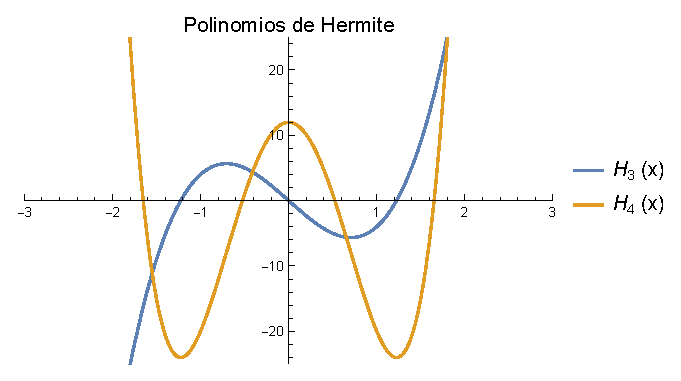
\includegraphics[scale=0.95]{Imagenes/Plot_Hermite_H3_H4.eps}
\end{figure}
\end{frame}

\subsection{Ejercicio 5}

\begin{frame}
\frametitle{Regla de recurrencia}
A partir de la siguiente regla de recurrencia que nos proporciona el polinomio de Hermite de orden $n + 1$, en términos de los dos polinomios precedentes:
\pause
\begin{align*}
H_{n+1} (x) = 2 \, x \, H_{n} (x) - 2 \, n \, H_{n - 1} (x)
\end{align*}
Con los resultados del ejercicio anterior, calcula los $H_{5} (x)$ y $H_{6} (x)$.
\end{frame}
\begin{frame}
\frametitle{Calculando $H_{5} (x)$}
Usando los resultados de $H_{3} (x)$ y $H_{4} (x)$ en conjunto con la regla de recurrencia:
\pause
\begin{eqnarray*}
\begin{aligned}
H_{5} &= 2 \, x \, H_{4} - 8 \, H_{3} = \\[0.5em] \pause
&= 2 \, x (12 - 48 \, x^{2} + 16 \, x^{4}) - 8 (- 12 \, x + 8 \, x^{3}) = \\[0.5em] \pause
&= 120 \, x - 160 \, x^{3} + 32 \, x^{5}
\end{aligned}
\end{eqnarray*}
\end{frame}
\begin{frame}
\frametitle{Calculando $H_{6} (x)$}
Usando los resultados de $H_{5} (x)$ y $H_{4} (x)$ en conjunto con la regla de recurrencia:
\pause
\begin{eqnarray*}
\begin{aligned}
H_{6} &= 2 \, x \, H_{5} - 10 \, H_{4} = \\[0.5em] \pause
&= 2 \, x (120 \, x - 160 \, x^{3} + 32 \, x^{5}) + \\[0.5em] 
&- 10 (12 - 48 \, x^{2} + 16 \, x^{4}) = \\[0.5em] \pause
&= - 120 + 720 \, x - 480 \, x^{4} + 64 \, x^{6}
\end{aligned}
\end{eqnarray*}
\end{frame}
\begin{frame}
\frametitle{Gráfica de $H_{5} (x)$ y $H_{6} (x)$}
\begin{figure}
  \centering
  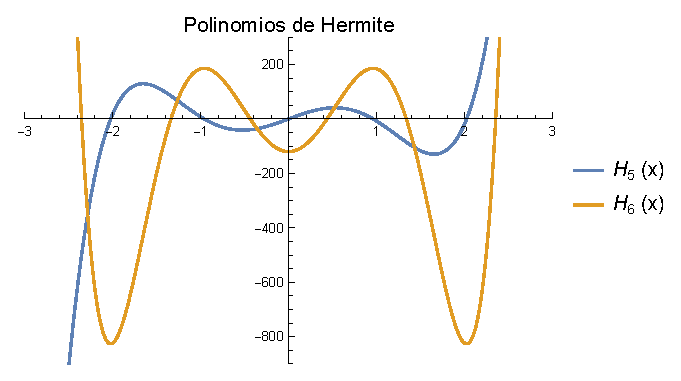
\includegraphics[scale=0.95]{Imagenes/Plot_Hermite_H5_H6.eps}
\end{figure}
\end{frame}
\end{document}